\documentclass[aspectratio=169, 10pt]{beamer}

% Kalbos ir šriftų nustatymai (Lietuvių kalbai)
\usepackage[utf8]{inputenc}
\usepackage[T1]{fontenc}
\usepackage[lithuanian]{babel}
\usepackage{lmodern}
\usepackage{amsmath, amssymb}
\usepackage{tikz}
\usetikzlibrary{trees, positioning, shapes}

% Beamer tema ir spalvos
\usetheme{Madrid}
\usecolortheme{whale}

% Navigacijos juostos paslėpimas
\setbeamertemplate{navigation symbols}{}

% Lietuviški aplinkų pavadinimai Beamer blokuose
\deftranslation[to=lithuanian]{Definition}{Apibrėžimas}
\deftranslation[to=lithuanian]{Example}{Pavyzdys}
\deftranslation[to=lithuanian]{Remark}{Pastaba}

% Paryškinto žodžio komanda (atitinkanti jūsų \vocab)
\newcommand{\vocab}[1]{\textbf{\color{structure.fg}#1}}

% Titulinio puslapio informacija
\title[Algebriniai reiškiniai]{Algebriniai reiškiniai}
\subtitle{Reiškinių tipai ir klasifikacija}
\author[A. Berniukevičius]{Andrius Berniukevičius}
\date{\today}

\begin{document}

% -----------------------------------------------------------------------------
% 1. Titulinis kadras
% -----------------------------------------------------------------------------
\begin{frame}
    \titlepage
\end{frame}

% -----------------------------------------------------------------------------
% 2. Įvadas ir pagrindinis apibrėžimas
% -----------------------------------------------------------------------------
\begin{frame}{Algebrinių reiškinių tipai}
    \vocab{Algebriniai reiškiniai} yra pagrindiniai matematikos kalbos elementai, kuriuose skaičiai ir kintamieji jungiami aritmetiniais veiksmais.
    
    \vspace{0.5cm}

    \begin{definition}[Algebrinis reiškinys]
        \vocab{Algebrinis reiškinys} – tai matematinis užrašas, sudarytas iš skaičių ir kintamųjų (raidžių), sujungtų aritmetinių veiksmų (sudėties, atimties, daugybos, dalybos, kėlimo laipsniu ar šaknies traukimo) ženklais. Reiškiniuose taip pat gali būti naudojami skliaustai.
    \end{definition}
\end{frame}

% -----------------------------------------------------------------------------
% 3. Veiksmų pavyzdžiai
% -----------------------------------------------------------------------------
\begin{frame}{Algebrinių reiškinių pavyzdžiai}
    \begin{example}[Pagrindiniai aritmetiniai veiksmai]
        \begin{itemize}
            \item \textbf{Sudėtis ir atimtis:} $3x + 5y - 7$
            \item \textbf{Daugyba:} $4a(a - 2b)$
            \item \textbf{Dalyba (trupmena):} $\dfrac{2x - 1}{x + 4}$
            \item \textbf{Kėlimas laipsniu:} $5x^4 - 2x^2 + 8$
            \item \textbf{Šaknies traukimas:} $\sqrt{x^2 + y^2}$
        \end{itemize}
    \end{example}
\end{frame}

% -----------------------------------------------------------------------------
% 4. Racionalieji ir irracionalieji reiškiniai
% -----------------------------------------------------------------------------
\begin{frame}{Racionalieji ir iracionalieji reiškiniai}
    Algebriniai reiškiniai skirstomi pagal tai, ar su kintamuoju atliekamas šaknies traukimo veiksmas arba kintamojo kėlimas trupmeniniu laipsniu:

    \begin{columns}[T]
        \begin{column}{0.48\textwidth}
            \begin{block}{Racionalus reiškinys}
                Atliekami tik sudėties, atimties, daugybos, dalybos ir kėlimo sveikuoju laipsniu veiksmai.
                \vfill
                \textbf{Pavyzdžiai:}
                \begin{itemize}
                    \item $3x^2 - 5$
                    \item $\frac{a+b}{c}$
                    \item $(x-2)(x+3)$
                \end{itemize}
            \end{block}
        \end{column}

        \begin{column}{0.48\textwidth}
            \begin{block}{Iracionalus reiškinys}
                Bent vienas kintamasis yra po šaknies ženklu arba keliamas trupmeniniu laipsniu.
                \vfill
                \textbf{Pavyzdžiai:}
                \begin{itemize}
                    \item $5\sqrt{a}+5b$
                    \item $\frac{4}{\sqrt[3]{x+y}}$
                    \item $x^{\frac{1}{3}} + 4x - 5$
                \end{itemize}
            \end{block}
        \end{column}
    \end{columns}

    \vspace{0.3cm}
    \begin{alertblock}{Pastaba}
        Reiškinys $\sqrt{5}x-3y$ \textbf{nėra} iracionalus, nes po šaknimi yra skaičius, o ne kintamasis.
    \end{alertblock}
\end{frame}

% -----------------------------------------------------------------------------
% 5. Sveikieji ir trupmeniniai reiškiniai
% -----------------------------------------------------------------------------
\begin{frame}{Sveikieji ir trupmeniniai reiškiniai}
    Racionalieji reiškiniai skirstomi pagal tai, ar juose yra \textbf{dalyba iš kintamojo}:

    \begin{columns}[T]
        \begin{column}{0.48\textwidth}
            \begin{block}{Sveikas reiškinys}
                Neturi dalybos iš kintamojo.
                \vfill
                \textbf{Pavyzdžiai:}
                \begin{itemize}
                    \item $7x^3 - 4x + 1$
                    \item $(a+2b)^3$
                    \item $\frac{x+3}{7}$
                \end{itemize}
            \end{block}
        \end{column}

        \begin{column}{0.48\textwidth}
            \begin{block}{Trupmeninis reiškinys}
                Yra dalyba iš kintamojo.
                \vfill
                \textbf{Pavyzdžiai:}
                \begin{itemize}
                    \item $\frac{5}{x} + x - 8$
                    \item $\frac{a+b}{a-b}$
                    \item $\frac{5}{x-3} + \frac{1}{x}$
                \end{itemize}
            \end{block}
        \end{column}
    \end{columns}

    \vspace{0.3cm}
    \begin{alertblock}{Pastaba}
        Reiškinyje $4x^{-2}$ dalybos tiesiogiai nematome, tačiau $4x^{-2} = 4 \cdot \frac{1}{x^2} = \frac{4}{x^2}$. Kadangi kintamasis yra vardiklyje – tai \textbf{trupmeninis reiškinys}.
    \end{alertblock}
\end{frame}

% -----------------------------------------------------------------------------
% 6. Klasifikacijos medis
% -----------------------------------------------------------------------------
\begin{frame}{Algebrinių reiškinių klasifikacijos medis}
    \centering
    \resizebox{\textwidth}{!}{%
    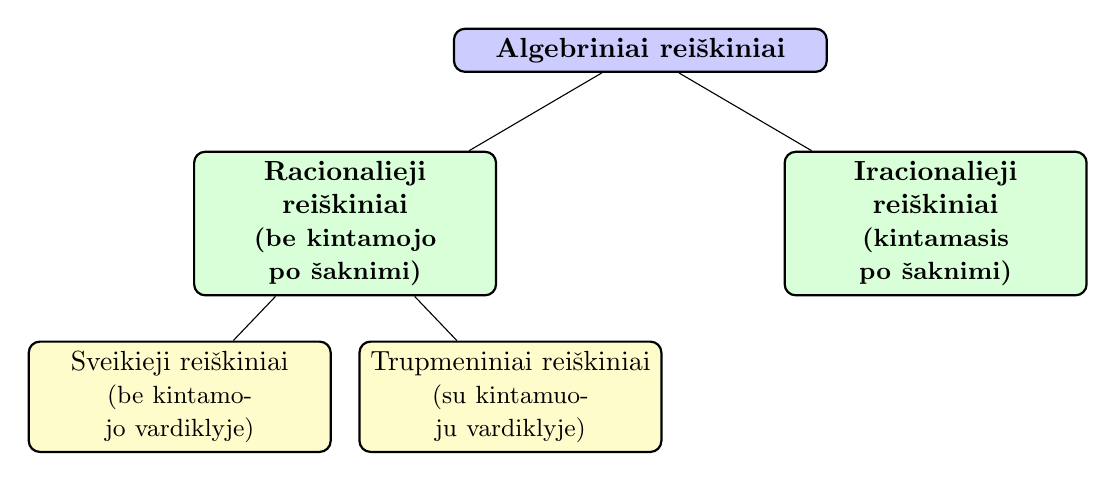
\begin{tikzpicture}[
      level distance=2.2cm,
      level 1/.style={sibling distance=7.5cm},
      level 2/.style={sibling distance=4.2cm},
      every node/.style={draw, rectangle, rounded corners, text width=3.6cm, align=center, thick},
      root/.style={fill=blue!20, text width=4.5cm, font=\bfseries},
      level1/.style={fill=green!15, font=\bfseries},
    level2/.style={fill=yellow!20}
    ]

      \node[root] {Algebriniai reiškiniai}
        child {node[level1] {Racionalieji reiškiniai \\ \small(be kintamojo po šaknimi)}
                    child {node[level2] {Sveikieji reiškiniai \\ \small(be kintamojo vardiklyje)}}
          child {node[level2] {Trupmeniniai reiškiniai \\ \small(su kintamuoju vardiklyje)}}
        }
        child {node[level1] {Iracionalieji reiškiniai \\ \small(kintamasis po šaknimi)}};

    \end{tikzpicture}
    }
\end{frame}

% -----------------------------------------------------------------------------
% 7. Uždaviniai (1 dalis)
% -----------------------------------------------------------------------------
\begin{frame}{Uždaviniai: Nustatykite reiškinio tipą (1/2)}
    Nustatykite reiškinių tipus: racionalus, iracionalus, sveikas arba trupmeninis. Reiškinys gali turėti daugiau nei vieną tipą.
    
    \vspace{0.3cm}
    \begin{columns}[T]
        \begin{column}{0.5\textwidth}
            \begin{enumerate}
                \item $7x^3 - x - 15$
                \item $\sqrt{ab} + 5$
                \item $\frac{7x}{3}$
                \item $\frac{5}{y^3}$
                \item $-6a^3bc^2$
                \item $x^2 + 2xy + y^2$
                \item $\sqrt{7}x - 2x^4$
                \item $5a^{-3}$
                \item $12$
                \item $\frac{x+3}{x-3}$
            \end{enumerate}
        \end{column}
        
        \begin{column}{0.5\textwidth}
            \begin{enumerate}
                \setcounter{enumi}{10}
                \item $y^{\frac{2}{3}} + 5y$
                \item $\frac{x-1}{3} + 4x$
                \item $abcd$
                \item $\frac{1}{\sqrt[3]{x}+2}$
                \item $(x-2)^3$
                \item $-\frac{3}{5}m^2n$
                \item $x + 8$
                \item $(x+3)(x-2)$
                \item $\frac{4}{x^2}$
                \item $a^2 - b^2$
            \end{enumerate}
        \end{column}
    \end{columns}
\end{frame}

% -----------------------------------------------------------------------------
% 8. Atsakymai
% -----------------------------------------------------------------------------
\begin{frame}{Atsakymai (1/2)}
    \begin{columns}[T]
        \begin{column}{0.5\textwidth}
            \small
            \begin{enumerate}
                \item Racionalus, sveikas
                \item Iracionalus
                \item Racionalus, sveikas
                \item Racionalus, trupmeninis
                \item Racionalus, sveikas
                \item Racionalus, sveikas
                \item Racionalus, sveikas
                \item Racionalus, trupmeninis
                \item Racionalus, sveikas
                \item Racionalus, trupmeninis
            \end{enumerate}
        \end{column}
        
        \begin{column}{0.5\textwidth}
            \small
            \begin{enumerate}
                \setcounter{enumi}{10}
                \item Iracionalus
                \item Racionalus, sveikas
                \item Racionalus, sveikas
                \item Iracionalus
                \item Racionalus, sveikas
                \item Racionalus, sveikas
                \item Racionalus, sveikas
                \item Racionalus, sveikas
                \item Racionalus, trupmeninis
                \item Racionalus, sveikas
            \end{enumerate}
        \end{column}
    \end{columns}
\end{frame}

\end{document}